%xelatex -output-directory=bin coding_style.tex
%Για να τρέξει σωστά το xelatex αφού του λέμε να βγάλει όλα τα αρχεία σε βοηθητικό αρχείο θα πρέπει να δημιουργήσουμε την ίδια δομή και στο φάκελo bin
%cp references.bib bin/references.bib
%cd bin/
%bibtex coding_style.aux
%cd .. 
%xelatex -output-directory=bin coding_style.tex
%xelatex -output-directory=bin coding_style.tex

\documentclass{assignment}

\usepackage{paralist} % για το περιβάλλον inparaenum που είναι οι λίστες μέσα στο κείμενο.
\usepackage{longtable} % για έναν μεγάλο πίνακα

\university{Πανεπιστήμιο Πειραιώς}{Πα.Πει.}
\school{Τμήμα Πληροφορικής}{Π.Μ.Σ. "Πληροφορική"}
\department{Πρόγραμμα Μεταπτυχιακών Σπουδών «Πληροφορική»}{}
%\cover{images/cover.jpg}{http://www.cyberciti.biz/faq/grub-boot-into-single-user-mode/}

\title{Στυλ προγραμματισμού}
%\projectlevel{Θέμα Εξαμήνου}
%\lesson{Εισαγωγή στην Επιστήμη των Υπολογιστών}{1}
\date{Αθήνα, 2014}

\author{Αναγνωστόπουλος Βασίλης - Θάνος}
%\register{ΜΠΠΛ13002}{1}



%\advisor{Τσακίρη Μαρία, Αναπληρώτρια Καθηγήτρια Ε.Μ.Π.}

\begin{document}

\maketitle

\setcounter{page}{1} 
\pagenumbering{roman}

\pagestyle{plain}


%\phantomsection \label{toc}
\addcontentsline{toc}{section}{Περιεχόμενα}
\tableofcontents
\newpage
\addcontentsline{toc}{section}{\listfigurename}
\listoffigures

\addcontentsline{toc}{section}{\listtablename}
\listoftables

\newpage

%\pagestyle{headings}
\pagestyle{fancy}
\setcounter{page}{1} 
\pagenumbering{arabic}

%\frontmatter 
%\pagestyle{plain}

%\cleardoublepage
%\phantomsection \label{toc}
%\addcontentsline{toc}{section}{Περιεχόμενα}
%\tableofcontents

%\newpage
%\cleardoublepage
%\phantomsection \label{listofphoto}
%\addcontentsline{toc}{chapter}{Κατάλογος εικόνων}
%\listofphotos

%\newpage
%\clearpage
%\phantomsection \label{listoffig}
%\addcontentsline{toc}{chapter}{\listfigurename}
%\listoffigures

%\newpage
%\clearpage
%\phantomsection \label{listoftab}
%\addcontentsline{toc}{chapter}{\listtablename}
%\listoftables
%\mtcaddchapter[\listtablename] % Λόγω του minitoc

%\mainmatter
%\pagestyle{headings}

%\chapter{Εισαγωγή}
\section{Εισαγωγή}

%\begin{homeworkProblem}
%test τεστ % Question

%\problemAnswer{ % Answer
%\begin{center}
%τεστ 2
%\end{center}

%τεστ 3
%}
%\end{homeworkProblem}

Στυλ προγραμματισμού (αγγλ. \en{Programming/Coding style} ή \en{Coding conventions}) είναι ένα σύνολο κανόνων ή κατευθυντήριων γραμμών που χρησιμοποιούνται κατά την σύνταξη του πηγαίου κώδικα ενός προγράμματος υπολογιστή σε μια συγκεκριμένη γλώσσα προγραμματισμού που συνιστά να χρησιμοποιούνται συγκεκριμένες πρακτικές και μέθοδοι για κάθε πτυχή ενός προγράμματος γραμμένο στην συγκεκριμένη γλώσσα. Ο σκοπός του προγραμματιστικού στυλ είναι να εξασφαλίσει ότι ο πηγαίος κώδικας είναι γραμμένος με τρόπο που βελτιώνει την αναγνωσιμότητα του καθώς και την συντηρησιμότητα του \cite{wiki:coding_convetions,wiki:Programming_style,ala2004supporting,Mohan,Oman}.

Το σύνολο των κανόνων που ισχύουν για την συγγραφή του πηγαίου κώδικα μπορούν να ταξινομηθούν σε 4 τομείς \cite{Mohan} (βλ. σχήμα \ref{fig:style_taxonomy}):
\begin{description}
\item [Τυπογραφικά στυλ: ] Κανόνες που αφορούν την διάταξη και την εμφάνιση του κώδικα καθώς και την χρήση σχολίων, αλλά όχι την εκτέλεση του προγράμματος.
\item [Γενικές πρακτικές προγραμματισμού: ] Κανόνες και κατευθυντήριες γραμμές σχετικά με την μεθοδολογία και την γλώσσα που χρησιμοποιούνται και επηρεάζουν τον πηγαίο κώδικα.
\item [Δομές ελέγχου: ] Κανόνες που επηρεάζουν την χρήση των αλγορίθμων καθώς και την υλοποίηση τους.
\item [Δομές πληροφοριών : ] Κανόνες που επηρεάζουν τις δομές δεδομένων, την ροή του προγράμματος καθώς και την αποθήκευση και χειρισμό της πληροφορίας.
\end{description}

\begin{figure}
\begin{center}
\resizebox*{16.5cm}{!}{
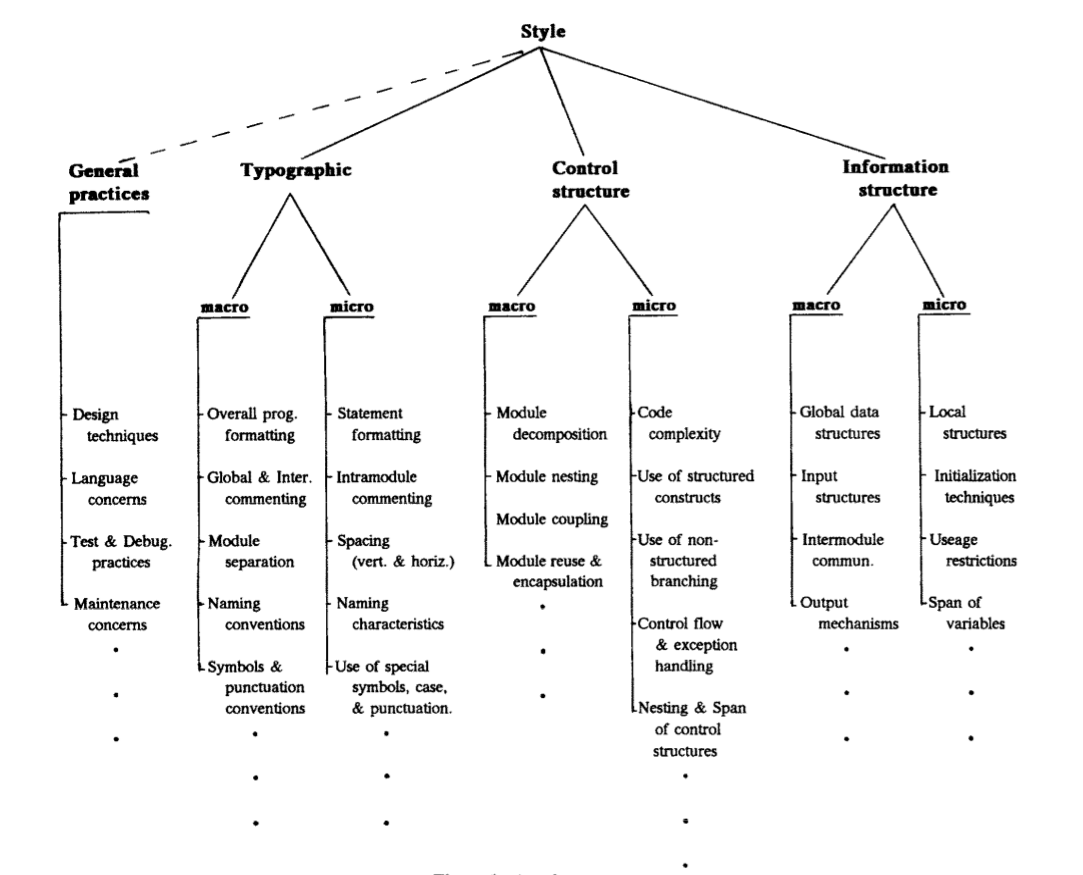
\includegraphics{images/style_taxonomy.png}}
\caption[Η ταξινόμηση του προγραμματιστικού στυλ]{Η ταξινόμηση του προγραμματιστικού στυλ \cite{Oman1991287}. }
\label{fig:style_taxonomy}
\end{center}
\end{figure}

%Οι παραπάνω τομείς περιλαμβάνουν συμβάσεις που καλύπτουν συνήθως
%\begin{inparaenum}[(i)]
%\item την οργάνωση των αρχείων (αγγλ. \en{file organization}), 
%\item τις εσοχές του κώδικα (αγγλ. \en{indentation}),
%\item τα σχόλια,
%\item τις δηλώσεις μεταβλητών και λοιπών στοιχείων,
%\item τα διαστήματα (αγγλ. \en{white space}),
%\item τις συμβάσεις για τα ονόματα (αγγλ. \en{naming conventions}),
%\item τις πρακτικές για καλό προγραμματισμό κ.λ.π. .
%\end{inparaenum}

Σε αυτή την εργασία θα αναπτυχθούν τα δύο πρώτα θέματα (τυπογραφικό στυλ και γενικές πρακτικές προγραμματισμού). Αυτές οι κατευθυντήριες γραμμές είναι για την διαρθρωτική ποιότητα του λογισμικού\footnote{Η διαρθρωτική ποιότητα του λογισμικού αναφέρεται στο πως οι μη -- λειτουργικές πτυχές του προγραμματισμού (όπως τα σχόλια, κ.λ.π) βοηθούν στην υλοποίηση των λειτουργικών πτυχών, όπως η αξιοπιστία του προγράμματος ή ευκολία στην συντήρηση του \cite{wiki:Software_quality}.} (αγγλ. \en{Software structural quality}). Προβάλλεται συχνά το επιχείρημα ότι ακολουθώντας ένα συγκεκριμένο προγραμματιστικό στυλ μπορεί να βοηθήσει στην ανάγνωση και κατανόηση του πηγαίου κώδικα, και επιπλέον βοηθά στην αποφυγή λαθών αλλά και στην βελτίωση της ποιότητας του πηγαίου κώδικα \cite{ala2004supporting,Ayerbe,Cox,WangZH08} (βλέπε ακόμα σχ. \ref{fig:coding_standard_to_software_quality}). Οι συμβάσεις που γίνονται όταν ακολουθείται ένα συγκεκριμένο στυλ προγραμματισμού βοηθά μόνο τους συντηρητές και τους διορθωτές του πηγαίου κώδικα ενός προγράμματος. Το προγραμματιστικό στυλ δεν επιβάλλεται από τους μεταγλωττιστές. Έτσι ένα πρόγραμμα το οποίο δεν ακολουθεί κάποιους ή όλους τους κανόνες δεν έχει καμία επίδραση στο εκτελέσιμο αρχείο του προγράμματος που δημιουργήθηκε από τον πηγαίο κώδικα \cite{wiki:coding_convetions,wiki:Programming_style}.

\begin{figure}
\begin{center}
\resizebox*{16.5cm}{!}{
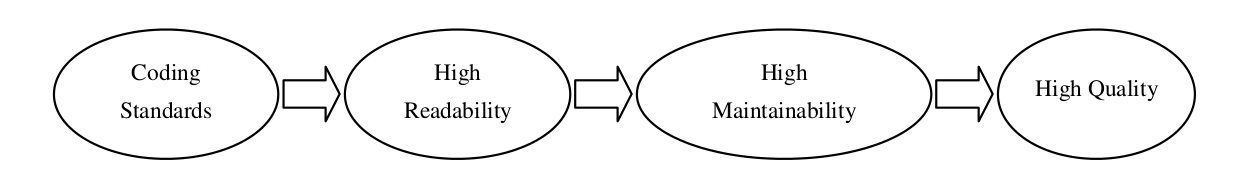
\includegraphics{images/coding_standard_to_software_quality.png}}
\caption[Η σχέση μεταξύ προγραμματιστικού στυλ και ποιότητας λογισμικο]{Η σχέση μεταξύ προγραμματιστικού στυλ και ποιότητας λογισμικού \cite{WangZH08}. }
\label{fig:coding_standard_to_software_quality}
\end{center}
\end{figure}

Το στυλ γραφής είναι ένα στοιχεία το οποίο συχνά παραβλέπεται αλλά είναι πολύ κρίσιμο χαρακτηριστικό της γραφής. Το ύφος της γραφής επηρεάζει άμεσα την αναγνωρισιμότητα και κατανόησης του τελικού προϊόντος. Έτσι ομοίως και το στυλ προγραμματισμού, που είναι η συγγραφή του πηγαίου κώδικα σε μία γλώσσα προγραμματισμού, ομοίως πάσχει από αυτή την παραμέληση. Τα προγράμματα πρέπει να είναι αναγνώσιμα και κατανοητά όχι μόνο από τις μηχανές αλλά ομοίως και από τον άνθρωπο. Η απαίτηση αυτή είναι σημαντική για τη δημιουργία ποιοτικών προϊόντων που ανταποκρίνονται όχι μόνο στις ανάγκες των χρηστών, αλλά επίσης μπορούν να αναπτυχθούν εντός προγράμματος και εκτιμώμενου κόστους. Η αποτελεσματική συγγραφή προγραμμάτων έχει ήδη ερευνηθεί από πολύ παλιά (\cite{Kernighan}) από τις πρώτες γλώσσες προγραμματισμού που υπήρχαν όπως η Fortan αλλά συνεχίζει να είναι ακόμα ένα φλέγον ζήτημα \cite{ala2004supporting,Kondoh200682}. 

Το στυλ προγραμματισμού που χρησιμοποιείται σε ένα συγκεκριμένο πρόγραμμα μπορεί να προέρχεται από τις συμβάσεις γραφής (αγγλ. \en{coding conventions}) που έχει κάνει μια εταιρεία ή κάποιος άλλος οργανισμός που ασχολείται με την συγγραφή κώδικά (π.χ. \cite{gnu_coding,site:gnu_style,site:google_cpp,
site:google_style,site:gnu_conventions,site:boost_guidelines,site:linux_style}) καθώς και τις προτιμήσεις του ίδιου του συγγραφέα. Υπάρχουν πολυάριθμες συμβάσεις γραφής που χρησιμοποιούνται για να διασφαλίσουν "συνεπή" (αγλλ. \en{consistent}) κώδικα. Οι συμβάσεις γραφής είναι σημαντικές στους προγραμματιστές διότι μπορούν να προσφέρουν αρκετά πλεονεκτήματα όπως \cite{wikibook:cpp_style,wiki:coding_convetions,sutter2004c++}:
%, οι οποίες βοηθούν στην βελτίωση της ποιότητας του κώδικα, συμπεριλαμβανομένου και την ορθότητα, αναγνωσιμότητα, την συντηρησιμότητα και την ταχύτητα \cite{wikibook:cpp_style}.

\begin{description}
\item [Συντήρηση λογισμικού (αγγλ. \en{Software maintenance}): ] Η  συντήρηση του λογισμικού αντιπροσωπεύει τουλάχιστον το 50\% του κόστους ζωής του λογισμικού\cite{Mohan}, ενώ σε άλλες έρευνες αναφέρετε ότι το 40\% με 80\% τους κόστους ζωής ενός λογισμικού πάει στην συντήρηση του κώδικα \cite{robert2003facts,wiki:coding_convetions}. Η μείωση, λοιπόν, του κόστους συντήρησης είναι ο πιο συχνά αναφερόμενος λόγος για την χρησιμοποίηση συμβάσεων γραφής. Σχεδόν κανένα λογισμικό δεν διατηρείται μόνο από τον αρχικό του δημιουργό. Έτσι οι συμβάσεις αυτές βοηθούν στην καλύτερη κατανόηση του κώδικα, επιτρέποντας και σε άλλους προγραμματιστές να συμμετέχουν στην επέκταση του κώδικα.
\item [Ποιότητα λογισμικού (αγγλ. \en{Software quality}): ] Η αξιολόγηση και η διόρθωση του κώδικα συχνά περιλαμβάνει την ανάγνωση του πηγαίου κώδικα από τρίτους. Εξ ορισμού, μόνο ο αρχικός συντάκτης έχει διαβάσει τον πηγαίο κώδικα πριν την αξιολόγηση του. Ο πηγαίος κώδικας ο οποίος τηρεί κάποιες συμβάσεις είναι πιο κατανοητός στους υπόλοιπους και επομένως η διαδικασία ανίχνευσής σφαλμάτων γίνεται πιο εύκολη. %Ακόμα και για τον αρχικό δημιουργό, όταν ο κώδικας τηρεί κάποιες συμβάσεις, διευκολύνεται η διαδικασία συντήρησης του πηγαίου κώδικα.
\item [Μειώνουν την πολυπλοκότητα: ] Όσο πιο σύνθετο είναι ένα έργο λογισμικού τόσο πιο πιθανό είναι να έχει σφάλματα. Οι σωστές συμβάσεις γραφής βοηθούν στην εύρεση αυτών των σφαλμάτων και στην μείωση της πολυπλοκότητας του πηγαίου κώδικα. %Η καλή μεθοδολογία και οι σωστές συμβάσεις γραφής μπορούν να χρησιμοποιηθούν έτσι ώστε η ποιότητα συγγραφής του κώδικα να είναι καλύτερη και ταυτόχρονα να μειωθεί ο χρόνος ανάπτυξης και συντήρησης της εφαρμογής.
\item [ Βελτιωμένη ταχύτητα ανάπτυξης και καλύτερη ομαδική εργασία: ] Οι προγραμματιστές δεν χρειάζεται να ξεκινούν πάντα από το μηδέν και έχουν μία στέρεα βάση για την ανάπτυξη του λογισμικού, ενώ ταυτόχρονα οι συμβάσεις συμβάλλουν στην μείωση των περιττών συζητήσεων σχετικά με ασήμαντα θέματα και διευκολύνουν στην συνεργασία μεταξύ των προγραμματιστών.
\end{description}

Τέλος τα πεδία που επηρεάζονται από την επιλογή ενός στυλ κώδικα φαίνονται συνοπτικά στο σχήμα \ref{fig:style_quality}.
%\begin{itemize}
%\item Η επαναχρησιμοποίηση του κώδικα  Re-usability
%\item Στην τεκμηρίωση του κώδικα  Self documenting code
%\item Στην συντηρισημότητα του κώδικα Maintainability
%\item Στην φορητότητα του κώδικα Portability
%\item Στην βελτιστοποίηση του κώδικα Optimization
%\item Στην ασφάλεια του κώδικα  Security
%\item Στην αποφυγή λαθών Error avoidance
%\item Internationalization
%\item Build process
%\end{itemize}
\begin{figure}
\begin{center}
\resizebox*{!}{8.5cm}{
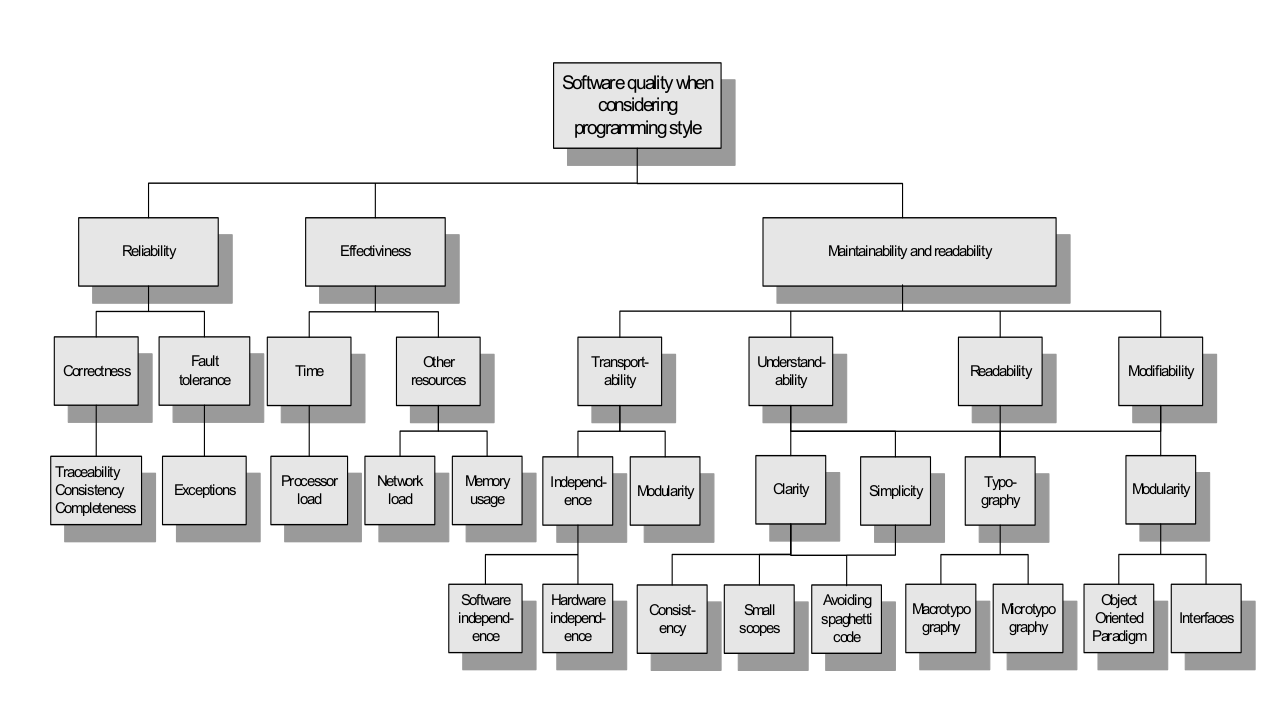
\includegraphics{images/style_quality.png}}
\caption[Τα πεδία που επηρεάζονται από την επιλογή ενός στυλ κώδικα]{Τα πεδία που επηρεάζονται από την επιλογή ενός στυλ κώδικα \cite{ala2004supporting}. }
\label{fig:style_quality}
\end{center}
\end{figure}

%\chapter{Στοιχεία καλού προγραμματιστικού στυλ}
%\section{Στοιχεία καλού προγραμματιστικού στυλ}

\section{Στοιχεία καλού προγραμματιστικού στυλ}
Το καλό στυλ στην συγγραφή κώδικα είναι υποκειμενικό θέμα και είναι δύσκολο να προσδιοριστεί. Παρόλα αυτά, υπάρχουν πολλά στοιχεία που είναι κοινά σε ένα μεγάλο αριθμό από στυλ προγραμματισμού. Σε αυτή την ενότητα θα παρατεθούν αυτά ακριβώς τα στοιχεία.

\subsection{Τυπογραφικό στυλ - Εμφάνιση κώδικα}

Το προγραμματιστικό στυλ συνήθως ασχολείται και με την οπτική εμφάνιση του πηγαίου κώδικα, με στόχο να απαιτείται λιγότερη προσπάθεια από τους προγραμματιστές για την αναγνώριση και την εξαγωγή χρήσιμων πληροφοριών από τον κώδικα . Όταν το πρόγραμμα ολοκληρωθεί, σπάνια ένας προγραμματιστής θα το διαβάσει από πάνω προς τα κάτω. Στον εντοπισμό σφαλμάτων και στην βελτιστοποίηση του προγράμματος, οι προγραμματιστές παραλείπουν συχνά μεγάλα τμήματα του κώδικα, προκειμένου να βρουν αυτό που ψάχνουν. Μια καλή αναλογία είναι αν συγκριθεί ο πηγαίος κώδικας με ένα λεξικό. Αν οι λέξεις σε ένα λεξικό δεν ήταν σε αλφαβητική σειρά και με έντονη γραφή τότε ο εντοπισμός μιας συγκεκριμένης λέξης θα ήταν πολύ δύσκολος. Ομοίως λοιπόν και στον πηγαίο κώδικα, η οπτική εμφάνιση του κώδικα βοηθά στην μετέπειτα επεξεργασία του \cite{wiki:Programming_style,site:codding_matters}.

Το τυπογραφικό στυλ έχει αποδειχθεί ότι επηρεάζει την δυνατότητα κατανόησης του πηγαίου κώδικα και η συνεπής εφαρμογή κάποιου τυπογραφικού στυλ ενισχύει την κατανόηση ενός προγράμματος \cite{Mohan}.

\subsubsection{Εσοχές του κώδικα}

Οι εσοχές στον κώδικα βοηθούν στον προσδιορισμό της ροής του προγράμματος. Συγκεκριμένα οι εσοχές χρησιμοποιούνται για να επιτρέψουν στον αναγνώστη του κώδικα να καθορίσει το επίπεδο ένθεσης μίας δήλωσης με μία ματιά και για να οριοθετήσουν λογικά μπλοκ κώδικα. Για να είναι χρήσιμες, οι εσοχές πρέπει να είναι συνεπής και να χρησιμοποιείται πάντα ο ίδιος αριθμός σε όλο το πρόγραμμα (ή τουλάχιστον στο ίδιο αρχείο του προγράμματος). Συνήθως αναφέρονται ότι οι εσοχές πρέπει να είναι μεταξύ 2 και 5 κενών \cite{wiki:Programming_style,site:codding_matters,sutter2004c++}. Παρακάτω ακουλουθούν δύο παραδείγματα που στο ένα χρησιμοποιούνται εσοχές ενώ στο άλλο όχι:

\begin{lstlisting}[style=cpp,caption= Παράδειγμα εσοχών (1), label=program:indentation(1)]
if (hours < 24 && minutes < 60 && seconds < 60)
{
    return true;
}
else
{
    return false;
}
\end{lstlisting}

και 

\begin{lstlisting}[style=cpp,caption= Παράδειγμα εσοχών (2), label=program:indentation(2)]
if  ( hours   < 24
   && minutes < 60
   && seconds < 60
)
{return    true
;}         else
{return   false
;}
\end{lstlisting}

Το πρώτο παράδειγμα είναι πιο εύκολο να διαβαστεί μιας και κάθε λογικό κομμάτι του κώδικα ξεχωρίζει. Επομένως οι εσοχές στον κώδικα βοηθούν στις εμφολιασμένες εντολές.


\subsubsection{Κατακόρυφη στοίχιση}

Είναι συχνά χρήσιμο να στοιχίζονται κατακόρυφα παρόμοια στοιχεία, για να φαίνονται τα τυπογραφικά σφάλματα \cite{wiki:Programming_style}. Για παράδειγμα:

\begin{lstlisting}[style=cpp, caption= Κατακόρυφη στοίχιση (1), label=program:vertical_aligment(1)]
$search = array('a', 'b', 'c', 'd', 'e');
$replacement = array('foo', 'bar', 'baz', 'quux');
\end{lstlisting}
 
και

\begin{lstlisting}[style=cpp, caption= Κατακόρυφη στοίχιση (2), label=program:vertical_aligment(2)]
$search      = array('a',   'b',   'c',   'd',   'e');
$replacement = array('foo', 'bar', 'baz', 'quux');
\end{lstlisting}

Το τελευταίο παράδειγμα κάνει δύο πράγματα διαισθητικά σαφές που πριν δεν ήταν:

\begin{itemize}
\item οι μεταβλητές \en{search} και \en{replacement} σχετίζονται μεταξύ τους
\item και υπάρχει ένας παραπάνω όρος στην μεταβλητή \en{search} από ότι στην μεταβλητή \en{replacement}. Αν πρόκειται για κάποιο σφάλμα είναι πιο πιθανόν τώρα να εντοπιστεί.
\end{itemize}

Ωστόσο, σημειώνετε ότι υπάρχουν πολλά επιχειρήματα κατά της κατακόρυφης στοίχισης όπως:

\begin{description}
\item [Ευθραυστότητα: ] Εάν ένας προγραμματιστής κάνει κάποια αλλαγή στον "πίνακα" και δεν τον τακτοποιήσει, έχει ως αποτέλεσμα την επιδείνωση της οπτικής εμφάνισης των στοιχείων, που γίνεται ακόμα χειρότερη με κάθε αλλαγή και
\item [Δυσκολία στην συντήρηση: ] Η μορφοποίηση του πίνακα απαιτεί περισσότερη προσπάθεια για να διατηρηθεί.
\end{description}

\subsubsection{Διαστήματα}

Το στυλ που σχετίζονται με τα διαστήματα \footnote{Τα κενά (διαστήματα), τα \en{tabs} και οι νέες γραμμές (αλλαγή γραμμής) ονομάζονται διαστήματα.} χρησιμοποιούνται για την ενίσχυση της αναγνωσιμότητας του πηγαίου κώδικα. Δεν υπάρχουν γνωστές μελέτες οι οποίες υποστηρίζουν ότι τα διαστήματα βοηθούν στην αναγνωσιμότητα του κώδικα αλλά από μία απλή σύγκριση του παρακάτω κώδικά φαίνεται ότι αμυδρά βοηθά στην καλύτερη κατανόηση του κώδικα. Για παράδειγμα \cite{wiki:Programming_style}: 

\begin{lstlisting}[style=cpp, caption= Διαστήματα (1), label=program:spaces(1)]
int i;
for(i=0;i<10;++i){
    printf("%d",i*i+i);
}
\end{lstlisting}

έναντι

\begin{lstlisting}[style=cpp, caption= Διαστήματα (2), label=program:spaces(2)]
int i;
for( i = 0; i < 10; ++i ) {
    printf( "%d", i * i + i );
}
\end{lstlisting}

Η χρήση των διαστημάτων στον πηγαίο κώδικα είναι όμοια με τους κανόνες της αγγλικής γλώσσας. Αυτό σημαίνει ότι \cite{site:codding_matters}:

\begin{enumerate}
\item Τα περισσότερα βασικά σύμβολα στις γλώσσες προγραμματισμού (π.χ. "=", "+", κ.λ.π.) θα πρέπει να έχουν τουλάχιστον ένα διάστημα πριν και ένα διάστημα μετά από αυτούς με τις παρακάτω εξαιρέσεις:
  \begin{enumerate}
  \item Δεν εμφανίζεται διάστημα πριν από κόμμα ή πριν από ερωτηματικό.
  \item Δεν εμφανίζεται διάστημα πριν ή μετά από τελεία.
  \item Δεν εμφανίζεται διάστημα μεταξύ των δυαδικών τελεστών (π.χ. "->", "++").
  \end{enumerate}
\item Περισσότερα από ένα κενά μπορούν να χρησιμοποιηθούν για την ευθυγράμμιση στοιχείων (όπως στην κατακόρυφη στοίχιση).
\item Κενές γραμμές θα πρέπει ακόμα να χρησιμοποιούνται για να τον διαχωρισμό λογικών μπλοκ κώδικάς, όπως
  \begin{enumerate}
  \item Στο αρχή του πηγαίου κώδικα όπου υπάρχουν οι ντιρεκτίβες \en{include, const, typedef} κ.λ.π. .
  \item και σε κομμάτια κώδικα που είναι εκτεταμένα και υπάρχουν μέσα τους ξεχωριστά τμήματα κώδικα και μπορούν να διαχωριστούν με μία κενή γραμμή.
  \end{enumerate}
\end{enumerate}


\subsubsection{Αγκύλες}

Στις γλώσσες προγραμματισμού που επιτρέπουν αγκύλες, έχει καταστεί κοινή πρακτική να χρησιμοποιούνται ακόμα και όταν η χρήση τους δεν είναι απαραίτητη. Η χρήση τους επιτρέπεται σε όλους τους βρόγχους επανάληψης και δομές ελέγχου. Για παράδειγμα:

\begin{lstlisting}[style=cpp, caption= Αγκύλες (1), label=program:brackets(1)]
for (i = 0 to 5) {
  print i * 2;
}
 
print "Ended loop";
\end{lstlisting}

Με την χρήση των αγκυλών αποτρέπονται λογικά σφάλματα, τα οποία συνήθως είναι και χρονοβόρα να εντοπιστούν, όπως όταν ένα ερωτηματικό τερματισμού εισάγεται κατά λάθος στον πηγαίο κώδικα (Αλγόριθμος \ref{program:brackets(2)})

\begin{lstlisting}[style=cpp, caption= Αγκύλες (2), label=program:brackets(2)]
 for (i = 0; i < 5; ++i);
    printf("\%d \n", i*2);    /* The incorrect indentation hides the fact 
                               that this line is not part of the loop body. */

 printf("Ended loop");
\end{lstlisting}

 
Ένα παρόμοιο λάθος είναι όταν προστίθεται μια επιπλέον γραμμή πριν την πρώτη γραμμή (αλγόριθμος \ref{program:brackets(3)})

\begin{lstlisting}[style=cpp, caption= Αγκύλες (3), label=program:brackets(3)]
 for (i = 0; i < 5; ++i)
    printf(logfile, "loop reached %d\n", i);
    printf("%d\n", i*2);    /* The incorrect indentation hides the fact 
                               that this line is not part of the loop body. */
  printf("Ended loop");
\end{lstlisting}

Γι` αυτό το λόγο έχει καθιερωθεί η χρήση των αγκυλών όπως στον αλγόριθμο \ref{program:brackets(4)}.
%An alternate and more traditional style is to explicitly indicate the nesting. This means that the opening and closing braces are in the same column:

\begin{lstlisting}[style=cpp, caption= Αγκύλες (4), label=program:brackets(4)]
for( index = 0 ; index < size ; ++index )
{
    arrayA[ index ] = arrayB[ index ] ;
}
\end{lstlisting}

Στον αλγόριθμο \ref{program:brackets(4)} φαίνεται σαφώς τόσο η αρχή όσο και το τέλος τους μπλοκ εντολών. Υπάρχουν και άλλες μεθοδολογίες τοποθέτησης των αγκυλών (όπως π.χ. η αρχική αγκύλη να μπαίνει αμέσως μετά την βρόγχο επανάληψης όπως και στον αλγόριθμο \ref{program:brackets(1)}) οι οποίες δεν διαφέρουν από τον τρόπο που περιγράφτηκε στον παραπάνω αλγόριθμο. Η μικροδιαφορές αυτές δεν επηρεάζουν την αναγνωσιμότητα του κώδικα αλλά θα πρέπει να υπάρχει συνέπεια στην χρήση των αγκυλών \cite{sutter2004c++}.

%\subsubsection{Στοίχιση και ευθυγράμμιση του κώδικα}

%Συμπυκνώνοντας λοιπόν τα άνωθεν έχουμε το παρακάτω παράδειγμα:

%\begin{lstlisting}[style=cpp, caption= Στοίχιση και ευθυγράμμιση του κώδικα (1), label=program:lining(1)]
%for(i=0;i<s;i++){a[i]=b[i];}
%\end{lstlisting}

%Ο στοιχισμένος κώδικας:

%\begin{lstlisting}[style=cpp, caption= Στοίχιση και ευθυγράμμιση του κώδικα (2), label=program:lining(2)]
%for( index = 0 ; index < size ; index++ )
%{
%    arrayA[ index ] = arrayB[ index ] ;
%}
%\end{lstlisting}

%Όπως παρατηρούμε, μπορεί ο καθένας να σαρώσει τον κώδικα και να δει τα μοτίβα που υπάρχουν στον κώδικα. Αυτό είναι πολύ σημαντικό, όχι μόνο για την κατανόηση του κώδικα, αλλά και για την εύρεση σφαλμάτων. Ο κώδικας που έχει πολλές περιττές παραλλαγές, είναι ο κώδικας στον οποίο χάνετε πολύ χρόνος εργασίας.


%\section{Γενικές πρακτικές προγραμματισμού}

\section{Γενικές πρακτικές προγραμματισμού}

%The essence of good programming style is communication. Good style in programming is roughly as difficult to learn as good style in English. In both cases, the document has no value if it does not convey its meaning to the reader. Any program that will be used must be maintained by somebody - and that somebody must be able to understand the code by reading it. Any program that needs debugging will be easier to debug if the creator carefully explains what's going on.

Κατά την διαδικασία εγγραφής του πηγαίου κώδικα, οι προγραμματιστές έχουν τρία βασικά εργαλεία για να δείξουν τις προθέσεις τους:
\begin{inparaenum}[(i)]
\item τα σχόλια (εξήγηση του πηγαίου κώδικα),
\item σαφή ονόματα μεταβλητών, σταθερών, συναρτήσεων κ.λ.π. (οι λέξεις του ίδιου του προγράμματος),
\item και το τυπογραφικό στυλ που αναπτύχθηκε στην προηγούμενη ενότητα.
\end{inparaenum}
Κάθε ένα από αυτά τα στοιχεία βοηθά στην επικοινωνία μεταξύ του του προγραμματιστή που έγραψε τον κώδικα και του προγραμματιστή που διαβάζει τον πηγαίο κώδικα.

Σε αυτή την ενότητα θα παρατεθούν γενικές πρακτικές προγραμματισμού οι οποίες βοηθούν στην καλύτερη κατανόηση του πηγαίου κώδικα. %Αυτές οι πρακτικές βοηθούν στην ελαχιστοποίηση του αριθμού των αγνώστων παραμέτρων και να μεγιστοποιήσουν τον αριθμό των γνωστών παραμέτρων \cite{wikibook:cpp_style}.

\subsection{Ονοματολογία (αγγλ. \en{Naming conventions})}

Η επιλογή των ονομάτων (των αρχείων, των μεταβλητών, των συναρτήσεων, κ.λ.π.) είναι από τα πιο σημαντικά στοιχεία που κάνουν τον πηγαίο κώδικα κατανοητό. Ο τρόπος με τον οποίο γράφουμε ένα όνομα μπορεί να μας πληροφορήσει άμεσα τί αντιπροσωπεύει η οντότητα αυτή όπως αν είναι μεταβλητή, συνάρτηση, σταθερά, κ.λ.π., χωρίς να χρειάζεται να αναζητήσουμε την δήλωση της οντότητας αυτής. Ακόμα τα ονόματα θα πρέπει να έχουν νόημα και να δίνουν στο προγραμματιστή την δυνατότητα να κατανοήσει και να διαβάσει τον πηγαίο κώδικα με ευκολία. Ένα όνομα το οποίο φαίνεται χαριτωμένο ή δακτυλογραφείται εύκολα μπορεί αργότερα να προκαλέσει προβλήματα σε κάποιον που προσπαθεί να κατανοήσει τον κώδικα. Ο πηγαίος κώδικας διαβάζεται πολλές φορές ενώ γράφεται μόνο μία. Γι` αυτό το λόγο η επιλογή της ονοματολογίας παίζει καθοριστικό ρόλο και το όνομα μιας μεταβλητής θα πρέπει να περιγράφει πλήρως και με ακρίβεια την μεταβλητή που αντιπροσωπεύει \cite{site:fx_alpha,site:taligent,site:google_style}.

Οι κανόνες της ονοματολογίας είναι αρκετά αυθαίρετοι, και γι` αυτό το λόγο οι κανόνες που παραθέτονται πιο κάτω είναι περισσότερο προτροπές ή συμβάσεις που έχουν υιοθετηθεί από ένα μεγάλο κομμάτι προγραμματιστών και όχι τόσο κανόνες. Αυτό που έχει σημασία είναι η συνέπεια τήρησης των οποίων αποφάσεων έχουν παρθεί ή έχουν χρησιμοποιήσει οι αρχικοί δημιουργοί του πηγαίου κώδικα \cite{site:google_style}.

\subsubsection[Γενικοί κανόνες]{Γενικοί κανόνες \cite{site:google_style,site:fx_alpha,site:geosoft,sutter2004c++,kernighan1988c}}

\begin{itemize}
\item Μια αποτελεσματική τεχνική για την εύρεση αντιπροσωπευτικών ονομάτων είναι η δήλωση με λόγια τι αντιπροσωπεύει η μεταβλητή. 

\item Τα ονόματα που επιλέγονται πρέπει να είναι αντιπροσωπευτικά, έτσι ώστε ο κώδικας να είναι άμεσα κατανοητός. Δεν θα πρέπει να χρησιμοποιούνται συντομογραφίες που είναι ασαφείς ή άγνωστες σε όσους διαβάζουν τον πηγαίο κώδικα για πρώτη φορά. Ακόμα δεν θα πρέπει να γίνονται συντμήσεις διαγράφοντας γράμματα από λέξεις. Πιο κάτω ακολουθούν μερικά "καλά" και "κακά" ονόματα μεταβλητών.

\begin{lstlisting}[style=cpp]
int price_count_reader;    // No abbreviation.
int num_errors;            // "num" is a widespread convention.
int num_dns_connections;   // Most people know what "DNS" stands for.

int n;                     // Meaningless.
int nerr;                  // Ambiguous abbreviation.
int n_comp_conns;          // Ambiguous abbreviation.
int wgc_connections;       // Only your group knows what this stands for.
int pc_reader;             // Lots of things can be abbreviated "pc".
int cstmr_id;              // Deletes internal letters.
int temp;                  // Is it temperature? Is it temporary?
\end{lstlisting}

\item Το μήκος μια μεταβλητής θα πρέπει να αντικατοπτρίζει και την εμβέλεια της. Μια τοπική μεταβλητή έχει περιορισμένη εμβέλεια, επομένως και το όνομα δεν χρειάζεται να είναι και πολύ περιγραφικό. Αντιθέτως μία παγκόσμια μεταβλητή, η εμβέλεια της οποίας είναι ευρεία, θα πρέπει να έχει ένα αντιπροσωπευτικό και περιγραφικό όνομα για να ξεχωρίζει. 

\item Οι συντομογραφίες και τα ακρωνύμια δεν πρέπει να είναι κεφαλαία όταν χρησιμοποιούνται ως ονόματα μεταβλητών.

\item Στους επαναληπτικούς βρόχους θα πρέπει να χρησιμοποιούνται ονομασίες με νόημα όπως φαίνεται και στο παρακάτω παράδειγμα:

{\begin{lstlisting}[style=cpp]
for (window_index = 0; window_index <= window_count; ++window_index) 
{ 
  ...  
}
\end{lstlisting}}


\end{itemize}

\subsubsection{Κανόνες ονοματολογίας}

Ο πίνακας \ref{table:naming_conventions} αναφέρει μερικές από τους πιο διαδεδομένους κανόνες που χρησιμοποιούνται στην ονοματολογία των οντοτήτων. Κατά κύριο λόγο περιλαμβάνονται κανόνες που εφαρμόζονται στην C++ αλλά μπορούν να γενικευτούν και στις υπόλοιπες γλώσσες προγραμματισμού.


%\begin{table}[htbp]
\begin{center}
\begin{longtable}{|m{0.11\textwidth}|m{0.45\textwidth}|m{0.40\textwidth}|}
\hline
Οντότητα & Περιγραφή & Παράδειγμα \\ \hline
\endfirsthead 

\hline Οντότητα & Περιγραφή & Παράδειγμα \endhead \hline

\hline \multicolumn{3}{|r|}{{Συνέχεια στην επόμενη σελίδα}} \\ \hline
\endfoot

\hline \hline
\endlastfoot


Αρχεία & 

{\begin{tabular}{@{}m{0.45\textwidth}@{}}
Για τα αρχεία διαλέγουμε ένα όνομα το οποίο αντικατοπτρίζει το περιεχόμενο του αρχείου.\\ \hline

Τα ονόματα των αρχείων θα πρέπει να είναι όλα πεζά και μπορεί να περιλαμβάνουν την κάτω παύλα (\_) ή την άνω παύλα (-). \\ \hline


Τα αρχεία προγραμμάτων της c++ θα πρέπει να τελειώνουν σε .cpp και της σε C θα πρέπει να τελειώνουν σε .c ενώ τα αρχεία κεφαλίδων θα πρέπει να τελειώνουν σε .h 
\end{tabular}} &
{\begin{lstlisting}[style=cpp, numbers=none]
my_useful_class.cpp
my-useful-class.cpp
myusefulclass.h
myusefulclass_test.h 
\end{lstlisting}}
\\ \hline

\en{Defines \& Macros} &

{Οι δηλώσεις επεξεργαστή και οι μακροεντολές θα πρέπει να είναι με κεφαλαία γράμματα. Ακόμα οι δηλώσεις επεξεργαστή για τα αρχεία θα πρέπει να τελειώνουν με κάτω παύλα (\_). 
%Include statements should be sorted and grouped. Sorted by their hierarchical position in the system with low level files included first. Leave an empty line between groups of include statements. 

} &

{\begin{lstlisting}[style=cpp, numbers=none]
#ifndef MODULE_NAME_FILE_NAME_HPP_
#define MODULE_NAME_FILE_NAME_HPP_

// the code

#endif // MODULE_NAME_FILE_NAME_HPP_

\end{lstlisting}}
\\ \hline


Με\-τα\-βλη\-τές &  

{\begin{tabular}{@{}m{0.45\textwidth}@{}}
Τα ονόματα των μεταβλητών (αγγλ. \en{variables}) είναι όλα πεζά, με παύλες μεταξύ των λέξεων. \\ \hline

Για τις παγκόσμιες μεταβλητές δεν υπάρχουν κάποιες ειδικές απαιτήσεις, μιας και η χρήση τους είναι σπάνια, αλλά σε κάθε περίπτωση αν χρησιμοποιείται κάποια, καλό θα ήταν να ξεχωρίζεται προτάσσοντας ένα g\_ ή κάποιο άλλο χαρακτηριστικό το οποίο θα τις ξεχωρίζει από τις τοπικές μεταβλητές.
\\ %\hline
%\en{Always using the unary scope resolution operator (::) to refer to global variables makesprograms easier to read and understand, because it makes it clear that you’re intending toaccess a global variable rather than a nonglobal variable.}
\end{tabular}} &

{\begin{lstlisting}[style=cpp, numbers=none]
string table_name;  // OK - uses underscore.

string tableName;   // Bad - mixed case.

int g_a_global_variable;
\end{lstlisting}}

\\ \hline

Συ\-να\-ρτή\-σεις &


{\begin{tabular}{@{}m{0.45\textwidth}@{}}

Οι συναρτήσεις (αγγλ. \en{functions}) θα πρέπει να είναι \en{camelCased}\footnotemark και οι μεταβλητές να είναι όλες πεζές, με κάτω παύλες (\_) μεταξύ των λέξεων.
\\ \hline

Ο τύπος επιστροφής της κάθε συνάρτησης θα πρέπει να τοποθετείται σε διαφορετική γραμμή \\ \hline

Πρέπει να διαλέγετε ως όνομα ένα ρήμα το οποίο αντανακλά την δράση της συνάρτησης. Καλό είναι να επιλέγονται ονόματα τα οποία αντανακλούν στοιχεία του προβλήματος και όχι την επίλυση του προβλήματος.
\end{tabular}} &

\footnotetext{CamelCase είναι η πρακτική της γραφής σύνθετων λέξεων ή φράσεων, έτσι ώστε κάθε λέξη ή σύντμηση να αρχίζει με ένα κεφαλαίο γράμμα. Αυτό επιτρέπει την μείωση του μεγέθους των φράσεων μιας και δεν χρησιμοποιούνται κενά ή κάποιοι άλλοι ειδικοί χαρακτήρες μεταξύ των λέξεων (π.χ. "\_" ανάμεσα στις λέξεις \cite{wiki:camelCase,site:yolinux}).}

{\begin{lstlisting}[style=cpp, numbers=none]
int
applyExample (int example_arg);

void
checkForErrors();
\end{lstlisting}}
\\ \hline

Ονόματα τύπων &

{\begin{tabular}{@{}m{0.45\textwidth}@{}}
Τα ονόματα των τύπων (αγλλ. \en{type names}) είναι \en{CamelCased}. Δηλαδή ξεκινούν με κεφαλαίο γράμμα και κάθε νέα λέξη να ξεκινά επίσης με κεφαλαίο, χωρίς να προηγείται κάτω παύλα (\_).
%Data members in structs should be named like regular variables without the trailing underscores that data members in classes have.
\end{tabular}} &

{\begin{lstlisting}[style=cpp, numbers=none]
// classes and structs
class UrlTable 
{ ...

class UrlTableTester 
{ ...

struct UrlTableProperties 
{
  string name;
  int num_entries;
}

// typedefs
typedef hash_map<UrlTableProperties *, string> PropertiesMap;

// enums
enum UrlTableErrors 
{ ...
\end{lstlisting}}
\\ \hline

Δομές &

{\begin{tabular}{@{}m{0.45\textwidth}@{}}
Τα μέλη μίας δομής πρέπει να ονομάζονται σαν κανονικές μεταβλητές. %χωρίς να ακολουθεί κάτω παύλα (\_)
\end{tabular}} &

{\begin{lstlisting}[style=cpp, numbers=none]
struct UrlTableProperties 
{
  string name;
  int num_entries;
}
\end{lstlisting}}
\\ \hline

Enum &

{\begin{tabular}{@{}m{0.45\textwidth}@{}}
Τα μέλη των απαριθμητών (αγγλ. \en{enumerations}) θα πρέπει να είναι κεφαλαία, με παύλες μεταξύ των λέξεων. Με τα κεφαλαία γράμματα οι σταθερές αυτές ξεχωρίζουν σε ένα πρόγραμμα και δεν μπερδεύονται με τις απλές μεταβλητές.
\end{tabular}} &

{\begin{lstlisting}[style=cpp, numbers=none]
enum Color 
{ 
  COLOR_RED, 
  COLOR_GREEN, 
  COLOR_BLUE 
};
\end{lstlisting}}
\\ \hline


Κλάσεις (1) 
&

{\begin{tabular}{@{}m{0.45\textwidth}@{}}
%Οι κλάσεις θα πρέπει να είναι \en{CamelCased}. Θα πρέπει να ξεκινούν με κεφαλαίο γράμμα και κάθε νέα λέξη να ξεκινά με κεφαλαίο. \\ \hline

Τα τμήματα μιας κλάσης πρέπει να ταξινομούνται ως: δημόσια, προστατευμένα (αγγλ.\en{public, protected}) και ιδιωτικά (αγλλ. \en{private}). Έτσι οι προγραμματιστές που θέλουν απλώς να χρησιμοποιήσουν την κλάση να μην χρειάζεται να διαβάζουν και τα ιδιωτικά μέλη της κλάσης. \\ \hline

Τα ιδιωτικά μέλη των κλάσεων είναι όπως και οι απλές μεταβλητές, μόνο που 
τελειώνουν με κάτω παύλα (\_). %Το πεδίο εφαρμογής μιας μεταβλητής είναι ένα από τα πιο σημαντικά χαρακτηριστικά της. 
Επισημαίνοντας το εύρος χρησιμοποιώντας κάτω παύλα καθιστά εύκολο τον διαχωρισμό τον μεταβλητών των κλάσεων από τοπικές μεταβλητές που χρησιμοποιούνται. %Αυτό είναι σημαντικό μιας και οι μεταβλητές των κλάσεων έχουν υψηλότερη σημασία από τις υπόλοιπες μεταβλητές και θα πρέπει να αντιμετωπίζονται με προσοχή από τους προγραμματιστές.

\end{tabular}} &

{\begin{lstlisting}[style=cpp, numbers=none]
class ExampleClass
{
    public:
    ...
    protected: 
    ... 

    private:
    int example_name_; 

}
\end{lstlisting}}
\\ \hline

Κλάσεις (2) &

{\begin{tabular}{@{}m{0.45\textwidth}@{}}


Μία κλάση πρέπει δηλώνετε σε ένα αρχείο επικεφαλίδας (αγγλ. \en{header file}) και να ορίζεται σε ένα πηγαίο αρχείο (αγγλ. \en{source file}) όπου τα ονόματα των αρχείων ταιριάζουν με το όνομα της κλάσης καθιστώντας εύκολη την εύρεση των αντίστοιχων αρχείων. Το αρχείο επικεφαλίδας πρέπει να ορίζει μία διεπαφή, και το πηγαίο αρχείο να την υλοποιεί. 
%\en{A class should be declared in a header file and defined in a source file where the name of the files match the name of the class. Makes it easy to find the associated files of a given class. An obvious exception is template classes that must be both declared and defined inside a .h file. The header files should declare an interface, the source file should implement it. When looking for an implementation, the programmer should always know that it is found in the source file.} 
\\ \hline
Τα αρχεία που υλοποιούν τις κλάσεις έχουν κατάληξη .hpp . \\ \hline

Οι συναρτήσεις ερωτημάτων (αγγλ. \en{accessors,mutators} ή συναρτήσεις \en{get} και \en{set}) πρέπει να ταιριάζουν με το όνομα της μεταβλητής που προελαύνουν. 
\end{tabular}} &

{\begin{lstlisting}[style=cpp, numbers=none]
class ExampleClass
{
  public:
  ...
  int 
  getNumEntries() const 
  { 
    return num_entries_; 
  }

  void 
  setNumEntries (int num_entries) 
  { 
    num_entries_ = num_entries; 
  }

  protected: 
  ... 

  private:
  int num_entries_;
  int example_name_; 

}
\end{lstlisting}}
\\ \hline

\caption{Ονοματολογια}
\label{table:naming_conventions}
%\end{table}
\end{longtable}
\end{center}


%Inline functions must be in a .h file. If your inline functions are very short, they should go directly into your .h file. However, if your inline functions include a lot of code, they may go into a third file that ends in -inl.h. In a class with a lot of inline code, your class could have three files:

%\begin{lstlisting}[style=cpp]
%url_table.h      // The class declaration.
%url_table.cc     // The class definition.
%url_table-inl.h  // Inline functions that include lots of code.
%\end{lstlisting}

\clearpage

\subsubsection{Υπο-φάκελοι}

Στον πίνακα \ref{table:subfolders} φαίνεται η τυπική δομή των φακέλων ενός τυπικού προγράμματος. Ομοίως και εδώ οι οι φάκελοι αυτοί είναι οι πιο χρησιμοποιούμενοι φάκελοι.

\begin{table}[htbp]
\begin{center}
\begin{tabular}{|m{0.20\textwidth}|m{0.75\textwidth}|}
\hline
Υπο-φάκελος   & Περιεχόμενα 	                         \\ \hline
include       & Τα αρχεία κεφαλίδων.                     \\ \hline
include/impl/ & Τα αρχεία που υλοποιούν τις κλάσεις.     \\ \hline
src 	      & Τα πηγαία αρχεία που χρειάζονται για 
                την μεταγλώττιση του προγράμματος.       \\ \hline
build 	      & Τα εκτελέσιμα αρχεία του προγράμματος.   \\ \hline
doc 	      & Τα αρχεία τεκμηρίωσης του προγράμματος.  \\ \hline

\end{tabular}
\end{center}
\caption[Υπο-φάκελοι του πηγαίου κώδικα]{Υπο-φάκελοι του πηγαίου κώδικα \cite{site:boost_guidelines,site:pcl}}
\label{table:subfolders}
\end{table}


\subsection[Σχολιασμός και τεκμηρίωση]{Σχολιασμός και τεκμηρίωση (αγγλ. \en{Commenting and Documentantion})\cite{wikibook:cpp_style}}

Η τεκμηρίωση και ο σχολιασμός του πηγαίου κώδικα είναι μία από τις πιο σημαντικές διαδικασίες κατά την παραγωγή του. Αν και δεν συνδέεται άμεσα με την λειτουργικότητα του κώδικα, συνδέεται έμμεσα με την δυνατότητα επέκτασης του, μιας και παρέχει με διορατικό τρόπο τις προθέσεις του αρχικού προγραμματιστή. %Αποτελείται από έγγραφα, όπως οι προδιαγραφές και περιγραφές του κώδικα. 

Κατάλληλα θέματα για την τεκμηρίωση συχνά περιλαμβάνουν:
\begin{itemize}
\item Γενική περιγραφή του προγράμματος. Πρέπει να περιλαμβάνει: 
  \begin{itemize}
  \item Μία επισκόπηση για το τον σκοπό που δημιουργήθηκε το πρόγραμμα.
  \item Ένα απλό παράδειγμα χρήσης του προγράμματος.
  \item Οδηγίες εκμάθησης για την βασική χρήση του προγράμματος.
  \end{itemize}
\item Τεκμηρίωση του κώδικα. Η τεκμηρίωση του κώδικα περιλαμβάνει:
  \begin{itemize}
    \item Περιγραφή των κλάσεων και των συναρτήσεων του προγράμματος.
    \item Την σχέση μεταξύ των κλάσεων και των συναρτήσεων.
    \item Για κάθε συνάρτηση, ανάλογα με την περίπτωση, μία περιγραφή, τις απαιτήσεις για την σωστή λειτουργία της, τα αποτελέσματα της, την τιμή που επιστρέφει καθώς και τυχόν σφάλματα που μπορεί να συμβούν.
    \item Εντοπισμό σφαλμάτων και στρατηγικές για την αποφυγή τους.
    \item Πως μεταγλωττίζεται και συνδέεται το πρόγραμμα.
    \item Η εκδοσή του προγράμματος και τυχόν αλλαγές που έχουν συμβεί.
    \item Αιτιολόγηση για τη λήψη αποφάσεων σχεδιασμού.
    \item Τυχόν ευχαριστίες.
  \end{itemize}
\end{itemize}

Με τα σχόλια και την τεκμηρίωση διασφαλίζεται ότι ο κώδικας έχει περιγραφτεί με επαρκείς λεπτομέρειες έτσι ώστε όταν κάποιος κοιτάζει τον πηγαίο κώδικα θα μπορεί εύκολα να καταλάβει το σχεδιασμό και το σκοπό του κώδικα \cite{wikibook:cpp_style}.

%to ensure that the code is written as desired. This form of comment is usually put in the code before the code is written. It serves as a means of ensuring that the code does what it is supposed to do.
\subsubsection[Γενικά σχόλια]{Γενικά σχόλια \cite{site:linux_style,sutter2004c++,wiki:coding_practices,site:google_style}}

\begin{itemize}

\item Σε γενικές γραμμές, χρειάζεται τα σχόλια να λένε \textbf{ΤΙ} κάνουν στον κώδικα και όχι \textbf{ΠΩΣ} το κάνουν.
%\item \en{Don't prescribe commenting styles (except where tools extract certain styles into documentation), but do write useful comments: Write code instead of comments wherepossible (e.g., see Item 16). Don't write comments that repeat the code; they getout of sync. Do write illuminating comments that explain approach and rationale}
\item Τα καλύτερα σχόλια στον πηγαίο κώδικα είναι ο ίδιος ο πηγαίος κώδικας. Γι` αυτό το λόγο ο κώδικας θα πρέπει να "αυτο-τεκμηριώνεται". Είναι προτιμητέο να εξηγείτε κάτι μέσα από τον ίδιο τον πηγαίο κώδικα (π.χ. με την χρήση κάποιου πολύπλοκου ονόματος μεταβλητής) παρά να χρησιμοποιούνται αργότερα σχόλια τα οποία εξηγούν τί κάνει ο συγκεκριμένος κώδικας.%\en{But remember: while comments are very important, the best code is self-documenting. Giving sensible names to types and variables is much better than using obscure names that you must then explain through comments.}
\item Σχόλια πρέπει να τοποθετούνται 
\begin{inparaenum}[(i)]
\item σε πολύπλοκα, 
\item μη προφανή, 
\item ενδιαφέροντα ή 
\item σημαντικά σημεία
\end{inparaenum} 
του πηγαίου κώδικα. Πριν από αυτά τα σημεία θα πρέπει να τοποθετούνται μικρά σχόλια τα οποία επεξηγούν τί κάνει ο κώδικας. Παραδείγματος χάρη: 
%\en{Also regarding complicated logic being used, it is a good practice to leave a comment "block" so that another programmer can understand what exactly is happening.}\item \en{In your implementation you should have comments in tricky, non-obvious, interesting, or important parts of your code. Tricky or complicated code blocks should have comments before them. Example:}

\begin{lstlisting}[style=cpp]
// Divide result by two, taking into account that x
// contains the carry from the add.
for (int i = 0; i < result->size(); i++) 
{
  x = (x << 8) + (*result)[i];
  (*result)[i] = x >> 1;
  x &= 1;
}
\end{lstlisting}

\item Αν τα σχόλια εκτείνονται σε αρκετές γραμμές, μπορεί η στοίχιση τους να τα κάνει πιο ευανάγνωστα. Παραδείγματος χάρη:

\begin{lstlisting}[style=cpp]
DoSomething();                  // Comment here so the comments line up.
DoSomethingElseThatIsLonger();  // Comment here so there are two spaces 
                                // between the code and the comment.
{ // One space before comment when opening a new scope is allowed,
  // thus the comment lines up with the following comments and code.
  DoSomethingElse();  // Two spaces before line comments normally.
}
DoSomething(); /* For trailing block comments, one space is fine. */
\end{lstlisting}
%\item \en{Pay attention to punctuation, spelling, and grammar; it is easier to read well-written comments than badly written ones. Comments should be as readable as narrative text, with proper capitalization and punctuation. In many cases, complete sentences are more readable than sentence fragments. Shorter comments, such as comments at the end of a line of code, can sometimes be less formal, but you should be consistent with your style.}

\end{itemize}

\subsubsection{Σχόλια οντοτήτων}

Ο πίνακας \ref{table:commeting_conventions} αναφέρει μερικούς από τους πιο διαδεδομένους τρόπους που χρησιμοποιούνται για να σχολιάσουν τις οντότητες του πηγαίου κώδικα.

\begin{center}
\begin{longtable}{|m{0.11\textwidth}|m{0.45\textwidth}|m{0.40\textwidth}|}
\hline
Οντότητα & Περιγραφή & Παράδειγμα \\ \hline
\endfirsthead 

\hline Οντότητα & Περιγραφή & Παράδειγμα \endhead \hline

\hline \multicolumn{3}{|r|}{{Συνέχεια στην επόμενη σελίδα}} \\ \hline
\endfoot

\hline \hline
\endlastfoot

Αρχεία & 

{\begin{tabular}{@{}m{0.45\textwidth}@{}}

Κάθε αρχείο πρέπει να περιέχει την άδεια χρήσης του πηγαίου κώδικα (π.χ. \en{Apache 2.0, BSD, LGPL, GPL}). Η επιλογή της κατάλληλης άδειας χρήσης είναι πολύπλοκη διαδικασία η οποία όμως δεν πρέπει να αμελείται. \\ \hline

Πρέπει να περιέχεται ο συγγραφέας του πηγαίου. \\ \hline

Κάθε αρχείο πρέπει να έχει ένα σχόλιο το οποίο περιγράφει τα περιεχόμενα του.
\end{tabular}} &
{\begin{lstlisting}[style=cpp, numbers=none]
/*
Copyright (c) 2013, Anagnostopoulos Vasilis-Thanos, Post-Graduate Student in University of Piraeus. All rights reserved.

Redistribution and use in source and binary forms, with or without modification,
are permitted provided that the following conditions are met:
  ...
*/

/*
This is a program that ...
*/
\end{lstlisting}}
\\ \hline

Με\-τα\-βλη\-τές & 

{\begin{tabular}{@{}m{0.45\textwidth}@{}}

Σε γενικές γραμμές το όνομα μίας μεταβλητής θα πρέπει να είναι αρκετά περιγραφικό ώστε να δίνει την δυνατότητα στον προγραμματιστή να καταλάβει για ποιο λόγο χρησιμοποιείται η συγκεκριμένη μεταβλητή. Σε ορισμένες περιπτώσεις, μερικά παραπάνω σχόλια χρειάζονται.% In general the actual name of the variable should be descriptive enough to give a good idea of what the variable is used for. In certain cases, more comments are required.} 
%\\ \hline
%\en{As with data members, all global variables should have a comment describing what they are and what they are used for. }
\end{tabular}} &
{\begin{lstlisting}[style=cpp, numbers=none]
// The total number of tests cases that we run through in this regression test.
const int k_num_test_cases = 6;
\end{lstlisting}}
\\ \hline

Συ\-να\-ρτή\-σεις (1) & 

{\begin{tabular}{@{}m{0.45\textwidth}@{}}

Κάθε δήλωση συνάρτησης θα πρέπει να έχει σχόλια τα οποία προηγούνται της συνάρτησης και περιγράφουν τί κάνει η συνάρτηση και πως να χρησιμοποιείται. Γενικά τα σχόλια στην δήλωση μίας συνάρτησης περιγράφουν την χρήση της συνάρτησης, ενώ τα σχόλια στην υλοποίηση μίας συνάρτησης περιγράφουν την λειτουργίας της.\\ \hline
Κατά την δήλωση μίας συνάρτησης πρέπει να αναφέρονται: 
\begin{itemize}
\item Οι μεταβλητές εισόδου και οι μεταβλητές που επιστρέφει η συνάρτηση.
%\item For class member functions: whether the object remembers reference arguments beyond the duration of the method call, and whether it will free them or not.
\item Εάν η συνάρτηση δεσμεύει μνήμη την οποία ο προγραμματιστής θα πρέπει να την αποδεσμεύσει (αυτό ισχύει σε γλώσσες που δεν έχουν συλλογή απορριμάτων (αγγλ. \en{garbage collection}) όπως η C++).
\item Εάν κάποια από τις μεταβλητές εισόδου ή εξόδου θα πρέπει να είναι δείκτης στο κενό. %Whether any of the arguments can be a null pointer.
\item Εάν υπάρχει οποιαδήποτε επίπτωση στην απόδοση με την χρησιμοποίηση της συνάρτησης. %If there are any performance implications of how a function is used.%\item If the function is re-entrant. What are its synchronization assumptions? 
\end{itemize} %\\ \hline 

\end{tabular}} &
{\begin{lstlisting}[style=cpp, numbers=none]
// Returns an iterator for this table.  It is the client's
// responsibility to delete the iterator when it is done with it,
// and it must not use the iterator once the GargantuanTable object
// on which the iterator was created has been deleted.
//
// The iterator is initially positioned at the beginning of the table.
//
// This method is equivalent to:
//    Iterator* iter = table->NewIterator();
//    iter->Seek("");
//    return iter;
// If you are going to immediately seek to another place in the
// returned iterator, it will be faster to use NewIterator()
// and avoid the extra seek.
Iterator* GetIterator() const;
\end{lstlisting}}

%//Or alternatively, constants or self-describing variables:
%
%const int kDefaultBaseValue = 10;
%const bool kFirstTimeCalling = false;
%Callback *null_callback = NULL;
%bool success = CalculateSomething(interesting_value,
%  kDefaultBaseValue,
%  kFirstTimeCalling,
%  null_callback);*
%
\\ \hline

Συ\-να\-ρτή\-σεις (2) & 

{\begin{tabular}{@{}m{0.45\textwidth}@{}}

Εάν υπάρχει κάποιο πολύπλοκο κομμάτι για το πως μίας συνάρτηση κάνει την δουλειά της τότε θα πρέπει να υπάρχει ένα επεξηγηματικό σχόλιο στην δήλωση της συνάρτησης το οποίο θα περιγράφει \begin{inparaenum}[(i)]
\item οποιοδήποτε κόλπα χρησιμοποιήθηκαν κατά την δημιουργία της συνάρτησης αυτής,
\item θα παρουσιάζει συνοπτικά τα βήματα που εκτελούνται κατά την λειτουργία της συνάρτησης
\item και θα εξηγεί γιατί δεν προτιμήθηκε κάποιος άλλος τρόπος υλοποίησης.
\end{inparaenum}.
%If there is anything tricky about how a function does its job, the function definition should have an explanatory comment. For example, in the definition comment you might describe any coding tricks you use, give an overview of the steps you go through, or explain why you chose to implement the function in the way you did rather than using a viable alternative. For instance, you might mention why it must acquire a lock for the first half of the function but why it is not needed for the second half.} 
\\ \hline

\item Όταν σε μία συνάρτηση περνιούνται σαν ορίσματα μεταβλητές boolean, ή ακέραιες μεταβλητές, ή κενοί δείκτες θα πρέπει να υπάρχουν σχόλια τα οποία θα επεξηγούν τί κάνουν αυτές οι τιμές.%\en{When you pass in a null pointer, boolean, or literal integer values to functions, you should consider adding a comment about what they are, or make your code self-documenting by using constants.}

\end{tabular}} &
{\begin{lstlisting}[style=cpp, numbers=none]
bool success = CalculateSomething(interesting_value,
  10,   // Default base value.
  false,// Not the first time we're calling this.
  NULL);// No callback.
\end{lstlisting}}
\\ \hline

Κλάσεις & 

{\begin{tabular}{@{}m{0.45\textwidth}@{}}

Κάθε κλάση πρέπει να έχει ένα συνοδευτικό σχόλιο το οποίο θα περιγράφει την κλάση και πως πρέπει να χρησιμοποιείται.\\ \hline %\en{Every class definition should have an accompanying comment that describes what it is for and how it should be used. Document the synchronization assumptions the class makes, if any. If an instance of the class can be accessed by multiple threads, take extra care to document the rules and invariants surrounding multithreaded use.} \\ \hline \en{When commenting constructors and destructors, remember that the person reading your code knows what constructors and destructors are for, so comments that just say something like "destroys this object" are not useful. Document what constructors do with their arguments (for example, if they take ownership of pointers), and what cleanup the destructor does. If this is trivial, just skip the comment. It is quite common for destructors not to have a header comment.} \\ \hline
Τα μέλη των συναρτήσεων θα πρέπει να έχουν ένα σχόλιο το οποίο περιγράφει την χρήση τους. Ακόμα αν μπορούν να λάβουν τιμές με ιδιαίτερη σημασία θα πρέπει να αναφέρονται στα σχόλια. \\ \hline % \en{Each class data member (also called an instance variable or member variable) should have a comment describing what it is used for. If the variable can take sentinel values with special meanings, such as a null pointer or -1, document this. }

Γενικά ένα αρχείο επικεφαλίδας θα περιγράφει τις κλάσεις που δηλώνονται μέσα στο αρχείο με μία επισκόπηση στο τί κάνει η κάθε κλάση και πως χρησιμοποιείται. Αντιθέτως ένα πηγαίο αρχείο πρέπει να περιέχει περισσότερες πληροφορίες για την υλοποίηση της κλάσης ή πολύπλοκων αλγορίθμων.
\end{tabular}} &
{\begin{lstlisting}[style=cpp, numbers=none]
// Iterates over the contents of a GargantuanTable.  Sample usage:
//    GargantuanTableIterator* iter = table->NewIterator();
//    for (iter->Seek("foo"); !iter->done(); iter->Next()) {
//      process(iter->key(), iter->value());
//    }
//    delete iter;
class GargantuanTableIterator 
{
  ...

  private:
  // Keeps track of the total number of entries in the table.
  // Used to ensure we do not go over the limit. -1 means
  // that we don't yet know how many entries the table has.
  int num_total_entries_;
};
\end{lstlisting}}
\\ \hline

\caption{Σχόλια}
\label{table:commeting_conventions}
%\end{table}
\end{longtable}
\end{center}

%Due to time restrictions or enthusiastic programmers who want immediate results for their code, commenting of code often takes a back seat. Programmers working as a team have found it better to leave comments behind since coding usually follows cycles, or more than one person may work on a particular module. Hence, it was made a "good practice" to leave comments behind in code.\cite{wikibook:cpp_style}


\subsection{Συνέπεια} 

Μία από τις πτυχές για την ποιοτική συγγραφή κώδικα είναι η συνέπεια (αγγλ. \en{Consistency}) στις αποφάσεις που έχουν ληφθεί , που συνεπάγεται ότι η η ποιότητα είναι αντιστρόφως ανάλογης των παρακλήσεων. Ο κώδικας που έχει πολλές περιττές παραλλαγές, είναι ο κώδικας στον οποίο χάνετε πολύ χρόνος εργασίας. Η συνέπεια είναι μια γενική αξία, και ως εκ τούτου, ακόμη και αν μία επιλογή θα μπορούσε να είναι καλύτερη σε μία συγκεκριμένη περίπτωση, το κόστος όμως για την συνέπεια πολλές φορές αντισταθμίζει τα τυχόν πλεονεκτήματα που ίσως υπάρχουν. Ωστόσο, μερικές φορές γίνονται εξαιρέσεις αν υπάρχουν ιδιαίτερα ελκυστικοί λόγοι ή σε προβλεπόμενες συνθήκες που έχουν θεσπιστεί κάποιες άλλες κατευθυντήριες γραμμές \cite{wiki:Programming_style}.

Συνέπεια στην συγγραφή του πηγαίου κώδικα είναι η χρησιμοποίηση των ίδιων προτύπων στις ίδιες καταστάσεις. Παραδείγματος χάρη, στην ονοματολογία η χρησιμοποίηση του ίδιου ονόματος, όταν παρουσιάζεται ο ίδιος τύπος κατάστασης. Αν χρησιμοποιούνται οι μεταβλητές \en{"i","index","inx"} κ.λ.π. στους βρόγχους επανάληψης τότε δεν έχουμε συνέπεια. Αντιθέτως, αν χρησιμοποιείται μόνο η μεταβλητή \en{"index"} τότε παράγεται κώδικας που είναι πολύ πιο απλώς και γρήγορος στην κατανόηση χωρίς περιττό "θόρυβο".\cite{wikibook:cpp_style}
%Meaningfulness is coding in a manner that conveys meaning. If a for loop uses just a letter 'i' for the index this is not very meaningful. If, however, the word 'index' is used this is much more meaningful.\cite{wikibook:cpp_style}
%One way in which we keep the code base manageable is by enforcing consistency. It is very important that any programmer be able to look at another's code and quickly understand it. Maintaining a uniform style and following conventions means that we can more easily use "pattern-matching" to infer what various symbols are and what invariants are true about them. Creating common, required idioms and patterns makes code much easier to understand. In some cases there might be good arguments for changing certain style rules, but we nonetheless keep things as they are in order to preserve consistency. \cite{site:google_style}


\subsection[Μαγικοί αριθμοί]{Μαγικοί αριθμοί \cite{wikibook:cpp_style,site:geosoft,kernighan1988c}}

Η πρακτική της ενσωμάτωσης δεδομένων εισόδου ή οποιοδήποτε άλλων δεδομένων στον πηγαίο κώδικα συναντάται στην βιβλιογραφία ως "μαγικοί αριθμοί" (αγγλ. \en{magic numbers} ή \en{hard coding}) και αποτελεί μία κακή προγραμματιστική τεχνική. Η χρησιμοποίηση τέτοιων αριθμών παράγουν κώδικα ο οποίος είναι δύσκολο να συντηρηθεί καθώς δεν δίνουν κάποια χρήσιμη πληροφορία σε κάποιον που διαβάζει τον πηγαίο κώδικα και είναι δύσκολο να αλλάξουν με συστηματικό τρόπο, αν είναι διεσπαρμένες μέσα στον πηγαίο κώδικα.

Εάν οι αριθμοί που χρησιμοποιούνται στον πηγαίο κώδικα δεν έχουν μία προφανή σημασία από μόνοι τους, τότε η αναγνωσιμότητα του πηγαίου κώδικα μπορεί να βελτιωθεί χρησιμοποιώντας μεταβλητές στην θέση των αριθμών. Εναλλακτικά μπορεί να χρησιμοποιηθεί και μία συνάρτηση που επιστρέφει την επιθυμητή τιμή. Στο πρόγραμμα \ref{program:hardcoding(1)} φαίνεται ένα ακριβώς τέτοιο παράδειγμα στο οποίο έχουν ενσωματωθεί "μαγικοί αριθμοί" μέσα στον πηγαίο κώδικα. 

\begin{lstlisting}[style=cpp,caption= Παράδειγμα "Μαγικών αριθμών" (1), label=program:hardcoding(1)]
#include <stdio.h>

/* print Fahrenheit-Celsius table */
int
main()
{
  int fahr;

  for (fahr = 0; fahr <= 300; fahr = fahr + 20)
    printf("%3d %6.1f\n", fahr, (5.0/9.0)*(fahr -32));

  return 0;
}
\end{lstlisting}

Αντιθέτως στο πρόγραμμα \ref{program:hardcoding(2)} που πλέον οι αριθμοί μέσα στο πηγαίο κώδικα έχουν αντικατασταθεί από μεταβλητές φαίνεται ξεκάθαρα η χρησιμότητα τους.

\begin{lstlisting}[style=cpp,caption= Παράδειγμα "Μαγικών αριθμών" (2), label=program:hardcoding(2)]
#include <stdio.h>
#define LOWER 0 /* lower limit of table */
#define UPPER 300 /* upper limit */
#define STEP 20 /* step size */

/* print Fahrenheit-Celsius table */
int
main()
{
  int fahr;

  for (fahr = LOWER; fahr <= UPPER; fahr = fahr + STEP)
    printf("%3d %6.1f\n", fahr, (5.0/9.0)*(fahr -32));

  return 0;
}
\end{lstlisting}

%The hard coding should be replaced by enumerated values or by \# defines ( soft coding ). Most compilers can handle enumerated values as non typed numbers and, as such, this is a safer method than using macros - \#defines. A soft coded project can be very quickly and safely updated. A hard coded project can be very time consuming and very dangerous to update.


\subsection[Σύγκριση με βάση το αριστερό μέλος]{Σύγκριση με βάση το αριστερό μέλος \cite{wikibook:cpp_style,deitel2011c++,programming2003high}} 

Στις γλώσσες προγραμματισμού που χρησιμοποιούν διαφορετικά σύμβολα για την ανάθεση τιμής (συνήθως ένα σύμβολο ίσον (\lstinline!=!) ) και για την σύγκριση  (συνήθως δύο ίσον (\lstinline!==!) ) (π.χ. C/C++, Java και η πλειοψηφία των γλωσσών τα τελευταία 15 χρόνια), και όπου οι αναθέσεις τιμών είναι συντακτικά σωστές μέσα σε δομές ελέγχου ή επαναληπτικούς βρόχους υπάρχει ένα πλεονέκτημα στην υιοθέτηση της σύγκρισης με βάσης το αριστερό μέρος και την τοποθέτηση των σταθερών ή των εκφράσεων προς τα αριστερά σε κάθε σύγκριση.

%In languages which use one symbol (typically a single equals sign, (=)) for assignment and another (typically two equals signs, (==) for comparison (e.g. C/C++, Java, ActionScript 3, PHP, Perl numeric context, and most languages in the last 15 years), and where assignments may be made within control structures, there is an advantage to adopting the left-hand comparison style: to place constants or expressions to the left in any comparison.


Στα προγράμματα \ref{program:left-comparison(1)} και \ref{program:left-comparison(2)} φαίνονται τα πλεονεκτήματα της υιοθέτησης της σύγκρισης με βάση το αριστερό μέλος. Και στις δύο περιπτώσεις θέλουμε να συγκρίνουμε την τιμή του \lstinline!a! με το \lstinline!42!. Στο πρώτο πρόγραμμα δεν υπάρχει κάποια διαφορά μιας και στις δύο περιπτώσεις η σύγκριση πραγματοποιείται σωστά. 

\begin{lstlisting}[style=cpp,caption= Παράδειγμα σύγκρισης με βάση το αριστερό μέλος (1), label=program:left-comparison(1)]
if (a == 42) { ... }  // A right-hand comparison checking if a equals 42.
if (42 == a) { ... }  // Recast, using the left-hand comparison style.
\end{lstlisting}

Η διαφορά και το πλεονέκτημα της σύγκρισης με βάση το αριστερό μέρος προκύπτει όταν ένας προγραμματιστής πληκτρολογήσει \lstinline!=! αντί για \lstinline!==!. 

\begin{lstlisting}[style=cpp,caption= Παράδειγμα σύγκρισης με βάση το αριστερό μέλος (2), label=program:left-comparison(2)]
if (a = 42) { ... }  // Inadvertent assignment which is often hard to debug
if (42 = a) { ... }  // Compile time error indicates source of error 
\end{lstlisting}

Στην πρώτη περίπτωση λοιπόν η τιμή του \lstinline!a! θα αλλάξει σε \lstinline!42!, με αποτέλεσμα ο κώδικας μέσα στην δομή ελέγχου \lstinline!if! να εκτελείται πάντα και καθώς η έκφραση αυτή είναι συντακτικά σωστή, το σφάλμα μπορεί να περάσει απαρατήρητο από το προγραμματιστή, και το λογισμικό μπορεί να κυκλοφορήσει με σφάλμα. Αντιθέτως στην δεύτερη περίπτωση θα έχουμε σφάλμα κατά την μεταγλώττιση του προγράμματος, καθώς δεν μπορούμε να αναθέσουμε τιμές σε αριθμητικές τιμές. Επομένως το σφάλμα θα διορθωθεί σίγουρα.


\section{Εφαρμογή και συμπεράσματα}

Αντί επιλόγου προτιμήθηκε να γραφτεί ένα πρότυπο προγράμματος το οποίο συνοψίζει όλες τις παραπάνω οδηγίες. Αυτό που θα ήθελα να τονίσω κλείνοντας είναι πως όλα τα παραπάνω δεν είναι αναγκαστικοί κανόνες αλλά περισσότερο προτροπές ή συμβάσεις που έχουν υιοθετηθεί από ένα μεγάλο κομμάτι προγραμματιστών. Δεν έχει τόσο σημασία αν κάποιος θα αφήσει δύο διαστήματα ή την αγκύλη θα την βάζει σε ξεχωριστή γραμμή όσο το να είναι συνεπής σε αυτές τις αποφάσεις.

Το νόημα της ύπαρξης κάποιων κατευθυντήριων γραμμών για την σύνταξη προγραμμάτων είναι για να μπορούν οι προγραμματιστές να έχουν ένα κοινό "λεξιλόγιο", ώστε να μπορούν να επικεντρωθούν σε αυτό που λέει το πρόγραμμα και όχι στο πως το λέει. 

Παρακάτω ακολουθεί ένα πρόγραμμα το οποίο τηρεί το σύνολο των παραπάνω κανόνων. 


\begin{lstlisting}[style=cpp]
/*
Copyright (c) 2013, Anagnostopoulos Vasilis-Thanos, Post-Graduate Student in University of Piraeus. All rights reserved.

Redistribution and use in source and binary forms, with or without modification,
are permitted provided that the following conditions are met:
  ...
*/

#ifndef TEST_H_
#define TEST_H_

#define SOME_MACRO_                            // all uppercase ending with trailing underscore

typedef double SomeType;                      // CamelCase, starting capital

/*
This is a class that ...
*/
class SomeClass 
{                             // camelcase, starting capital
  public:
    void method();
    Real anotherMethod(Real x,                // camelcase, starting lowercase
                       Real y) const;
    void setMember(Real);                     // setter, leading "set"

  private:
    //Some comment describing the variables
    Real member_;                             // all lowercase with underscore between the words
    Integer another_member_;                  // trailing underscore
};

struct SomeStruct 
{
  Real foo_foo;                             // struct members:
  Integer bar;                              // no trailing underscore
};

/*
This is a function that ...
*/
Size 
someFunction(Real parameter,             // one parameter per line,
             Real another_parameter)      // camelCase, starting lowercase
{    
  Real local_variable = 0.0;
  if (condition)
  {                                         // brackets here...
      local_variable += 3.14159;
  } 
  else  
  {                                         // ...here...
      local_variable -= 2.71828;
  }                                         // ...and here.
  return 42;
}

#endif // TEST_H_
\end{lstlisting}




%\subsection{Keep the code simple}

%\subsection{Portability}


%\section{Δομές Ελέγχου και πληροφοριών}

%http://en.wikipedia.org/wiki/Anti-pattern#Software_engineering
%Να το κοιτάξω και αυτό

%\subsection{Safe coding}

%Implicit test for 0 should not be used other than for boolean variables and pointers.  It is not necessarily defined by the C++ standard that ints and floats 0 are implemented as binary 0. Also, by using an explicit test the statement gives an immediate clue of the type being tested. It is common also to suggest that pointers shouldn't test implicitly for 0 either, i.e. if (line == 0) instead of if (line). The latter is regarded so common in C/C++ however that it can be used. 

%Safe coding conventions help to catch errors.\cite{site:fx_alpha}

%    Clearly document any assumptions made by functions in the comment block that precedes the function body.
%    Be sure that every variable is initialized before use.
%    Avoid type-casts whenever possible. When casting is unavoidable, an explicit cast is preferred over an implicit (compiler provided) one.
%    Select restrictive argument types. This primarily includes the keywords unsigned and const, and using enumerations in preference to simple integers.
%    Be sure that all functions have an explicit return type, even if that type is void.
%    "A ... function must never return a reference or a pointer to a local variable." (Ellemtel Rule 34.) This rule applies to all C functions and to public C++ functions.
%    "Do not write code which is dependent on the lifetime of a temporary object." (Ellemtel Prt. Rec. 16.)
%    "Do not allocate memory and expect that someone else will deallocate it later." (Ellemtel Rec. 58.)
%    "Always assign a new value to a pointer that points to deallocated memory." (Ellemtel Rec. 59.)
%    "Always use inclusive lower limits and exclusive upper limits." (Ellemtel Rec. 52.) Also see Koenig Sec. 3.6 and Formatting point f in Section 8.
%    If a C function has no parameters, use the keyword void to ensure consistency with C++. For example, int fnThatTakesNoParams(void);
%    Use an explicit status parameter for a function that returns a status. Do not overload data-passing parameters or the function return value. That is, do not use a special, reserved data value to indicate a return status.
%    Other error handling conventions are yet to be determined. 

%\cite{sutter2004c++}
%Compile cleanly at high warning levels.
%Take warnings to heart: Use your compiler's highest warning level. Require clean (warning-free) builds. Understand all warnings. Eliminate warnings by changing your code, not by reducing the warning level.

%Start with a clean slate: Uninitialized variables are a common source of bugs in C and C++ programs. Avoid such bugs by being disciplined about cleaning memory before you use it; initialize variables upon definition.

%Αυτό το κομμάτι είναι και το πιο σημαντικό στο programming style αλλά λόγω έλλειψης πείρας και κατανόησης των εννιοίων θα παραπείνουμε στο επιφανειακό κομμάτι και ο αναγνώστης που ενδιαφέρετε περισσότερο θα πρέπει να αναζητήσει μόνος τους λεπτομέρειες. \cite{programming2013high,programming2003high,gnu_coding,sutter2004c++}

%Do not write code that expects floating point calculations to yield exact results.

%Equivalence tests for floating point values should use <, <=, >, >=, and not use == or !=. Floating point representations are platform dependent, so it is necessary to avoid exact comparisons.
%\begin{lstlisting}[style=cpp]
%bool double_equal( const double a, const double b )
%{
%const double scale = ( std::fabs( a ) + std::fabs( b ) ) / 2.0;
%return std::fabs( a - b ) <= ( std::numeric_limits<double>::epsilon()
%* scale );
%}
%void foo( double f )
%{
%if ( f != 3.142 )
%{}
%// avoid
%if ( double_equal( f, 3.142 ) ) // prefer
%{}
%}
%\end{lstlisting}





%\cite{kernighan1988c}
%Because the else part of an if-else is optional,there is an ambiguity when an else if omitted from a nested if sequence. This is resolved by associating the else with the closest previous else-less if. For example, in

%if (n > 0)
%  if (a > b)
%    z = a;
%  else
%    z = b;
%else goes to the inner if,
%the
%as we have shown by indentation. If that isn't what you want, braces must be used to force the proper association:
%if (n > 0) {
%  if (a > b)
%    z = a;
%}
%else
%  z = b;
%The ambiguity is especially pernicious in situations like this:
%if (n > 0)
%  for (i = 0; i < n; i++)
%    if (s[i] > 0) {
%      printf("...");
%      return i;
%    }
%else /* WRONG */
%  printf("error -- n is negative\n");

%The indentation shows unequivocally what you want, but the compiler doesn't get the message, and associates the else with the inner if. This kind of bug can be hard to find; it's a good idea to use braces when there are nested ifs.


%Compiler Options

%The compiler must build cleanly with -Wall -Wextra. 


% Να βάλω τπτ για το valgrind


%\chapter{C++ Programming Style}\cite{wikibook:cpp_programming}


%The use of a guide or set of convention gives programmers a set of rules for code normalization or coding style that establishes how to format code, name variables, place comments or any other non language dependent structural decision that is used on the code. This is very important, as you share a project with others. Agreeing to a common set of coding standards and recommendations saves time and effort, by enabling a greater understandings and transparency of the code base, providing a common ground for undocumented structures, making for easy debugging, and increasing code maintainability. These rules may also be referred to as Source Code Style, Code Conventions, Coding Standards or a variation of those.


%\cite{site:google_style}
% All header files should have \#define guards to prevent multiple inclusion. The format of the symbol name should be <PROJECT>\_<PATH>\_<FILE>\_H\_.

%To guarantee uniqueness, they should be based on the full path in a project's source tree. For example, the file foo/src/bar/baz.h in project foo should have the following guard:

%\begin{lstlisting}[style=cpp]
%#ifndef FOO_BAR_BAZ_H_
%#define FOO_BAR_BAZ_H_

%...

%#endif  // FOO_BAR_BAZ_H_
%\end{lstlisting}


%\en{Class variables should never be declared public. The concept of C++ information hiding and encapsulation is violated by public variables. Use private variables and access functions instead. One exception to this rule is when the class is essentially a data structure, with no behavior (equivalent to a C struct). In this case it is appropriate to make the class' instance variables public [2]. Note that structs are kept in C++ for compatibility with C only, and avoiding them increases the readability of the code by reducing the number of constructs used. Use a class instead. }



%Always code as if the guy who ends up maintaining your code will be a violent psychopath who knows where you live. -- Martin Golding



\phantomsection \label{Βιβλιογραφία}
\addcontentsline{toc}{section}{Βιβλιογραφία}
%\mtcaddchapter[Βιβλιογραφία] % Λόγω του minitoc
\bibliographystyle{plain}
\bibliography{references}


\end{document}


